\begin{wrapfigure}[0]{r}[9pt]{0cm}
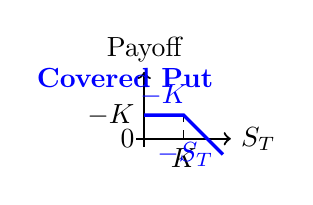
\begin{tikzpicture}[scale=1]
    % --- Define Coordinates and Parameters ---
    \def\K{0.5}        % Strike price K
    \def\maxST{1}    % Max S_T range
    \def\yAxisLevel{-0.8} % The y-coordinate where the x-axis will be drawn (visually "0")

    % --- Draw Axes ---
    % X axis (S_T) - shifted down to \yAxisLevel
    \draw[->, thick] (-0.1, \yAxisLevel) -- (\maxST + 0.1, \yAxisLevel) node[right] {$S_T$};
    % Y axis (Payoff) - spans from below the new x-axis to above the true y=0
    \draw[->, thick] (0, \yAxisLevel - 0.1) -- (0, 0.05) node[above] {Payoff};

    % --- Draw Auxiliary Lines and Labels ---
    % Mark "0" on the y-axis at the new x-axis level
    \node[left] at (0, \yAxisLevel) {0};

    % Mark K on the new x-axis, extend dashed line up to the payoff curve
    \draw[dashed, thin] (\K, \yAxisLevel) node[below] {$K$} -- (\K, -\K);

    % Mark -K on the y-axis (at its true negative value)
    \draw[dashed, thin] (0, -\K) node[left] {$-K$} -- (\K, -\K);


    % --- Draw Final Covered Put Payoff (Blue Thick Line) ---
    % The coordinates are relative to the true (0,0), so they remain the same.
    % When S_T < K: Payoff = -K
    % When S_T >= K: Payoff = -S_T
    \draw[blue, very thick] (0, -\K) -- (\K, -\K) -- (\maxST, -\maxST);

    % --- Add Simplified Labels ---
    % Label for the horizontal segment
    \node[blue, above] at (\K/2, -\K) {$-K$};
    % Label for the sloped segment
    \node[blue, left] at (\maxST, -\maxST) {$-S_T$};
    % Main Title Label
    \node[blue, anchor=south east, font=\bfseries,yshift=15pt] at (\maxST, \yAxisLevel) {Covered Put};

\end{tikzpicture}
\end{wrapfigure}